

\tikzset{every picture/.style={line width=0.75pt}} %set default line width to 0.75pt        

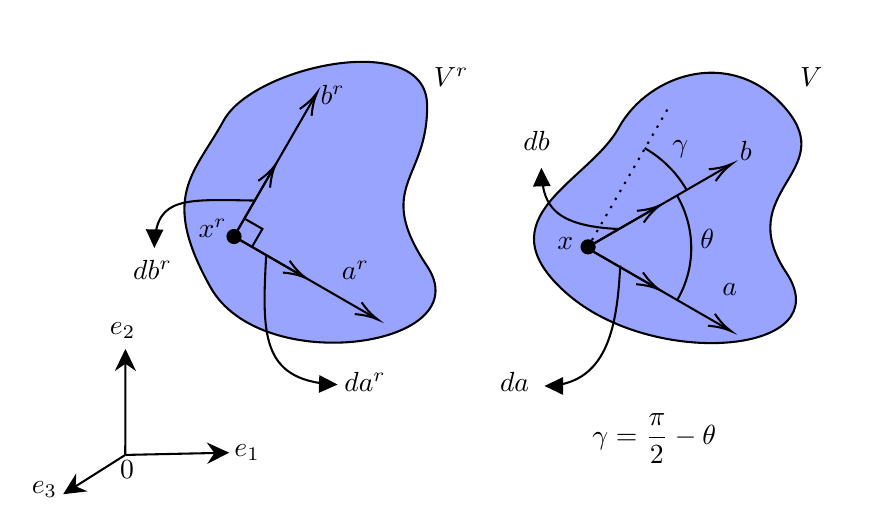
\begin{tikzpicture}[x=0.75pt,y=0.75pt,yscale=-1,xscale=1]
%uncomment if require: \path (0,249); %set diagram left start at 0, and has height of 249

%Shape: Polygon Curved [id:ds37090510589079506] 
\draw  [fill={rgb, 255:red, 0; green, 27; blue, 255 }  ,fill opacity=0.4 ] (443.7,47.62) .. controls (458.13,21.39) and (498.78,8.28) .. (524.35,38.7) .. controls (549.92,69.12) and (498.12,78.04) .. (524.35,117.38) .. controls (550.58,156.72) and (460.75,164.32) .. (418.79,127.61) .. controls (376.83,90.89) and (429.28,73.84) .. (443.7,47.62) -- cycle ;
%Shape: Regular Polygon [id:dp5727859442047756] 
\draw  [fill={rgb, 255:red, 0; green, 27; blue, 255 }  ,fill opacity=0.4 ] (253.42,44.02) .. controls (267.69,18.08) and (350.69,-0.07) .. (351.33,36.5) .. controls (351.98,73.07) and (325.4,75.4) .. (351.33,114.31) .. controls (377.27,153.21) and (271.58,168.52) .. (246.94,124.42) .. controls (222.3,80.33) and (239.16,69.96) .. (253.42,44.02) -- cycle ;
%Straight Lines [id:da34741946249595057] 
\draw    (205.92,205.28) -- (206,157.2) ;
\draw [shift={(206,154.2)}, rotate = 450.09] [fill={rgb, 255:red, 0; green, 0; blue, 0 }  ][line width=0.08]  [draw opacity=0] (10.72,-5.15) -- (0,0) -- (10.72,5.15) -- (7.12,0) -- cycle    ;
%Straight Lines [id:da35183475808822884] 
\draw    (205.92,205.28) -- (253,204.26) ;
\draw [shift={(256,204.2)}, rotate = 538.76] [fill={rgb, 255:red, 0; green, 0; blue, 0 }  ][line width=0.08]  [draw opacity=0] (10.72,-5.15) -- (0,0) -- (10.72,5.15) -- (7.12,0) -- cycle    ;
%Straight Lines [id:da3444772189505243] 
\draw    (205.92,205.28) -- (178.54,222.6) ;
\draw [shift={(176,224.2)}, rotate = 327.69] [fill={rgb, 255:red, 0; green, 0; blue, 0 }  ][line width=0.08]  [draw opacity=0] (10.72,-5.15) -- (0,0) -- (10.72,5.15) -- (7.12,0) -- cycle    ;
%Shape: Ellipse [id:dp7016292540356281] 
\draw  [fill={rgb, 255:red, 0; green, 0; blue, 0 }  ,fill opacity=1 ] (426.03,103.73) .. controls (426.75,102.14) and (428.61,101.44) .. (430.2,102.16) .. controls (431.78,102.88) and (432.48,104.74) .. (431.76,106.33) .. controls (431.05,107.91) and (429.18,108.61) .. (427.6,107.89) .. controls (426.01,107.18) and (425.31,105.31) .. (426.03,103.73) -- cycle ;
%Curve Lines [id:da9364210310002001] 
\draw    (443.9,96.45) .. controls (412.41,95.04) and (407.35,84.85) .. (406.51,69.88) ;
\draw [shift={(406.4,66.95)}, rotate = 448.57] [fill={rgb, 255:red, 0; green, 0; blue, 0 }  ][line width=0.08]  [draw opacity=0] (8.93,-4.29) -- (0,0) -- (8.93,4.29) -- cycle    ;
%Straight Lines [id:da07400897737098244] 
\draw    (258.32,100.05) -- (297.32,32.5) ;
\draw [shift={(298.32,30.77)}, rotate = 480] [color={rgb, 255:red, 0; green, 0; blue, 0 }  ][line width=0.75]    (10.93,-3.29) .. controls (6.95,-1.4) and (3.31,-0.3) .. (0,0) .. controls (3.31,0.3) and (6.95,1.4) .. (10.93,3.29)   ;
%Straight Lines [id:da013971101698424304] 
\draw    (258.32,100.05) -- (325.87,139.05) ;
\draw [shift={(327.6,140.05)}, rotate = 210] [color={rgb, 255:red, 0; green, 0; blue, 0 }  ][line width=0.75]    (10.93,-3.29) .. controls (6.95,-1.4) and (3.31,-0.3) .. (0,0) .. controls (3.31,0.3) and (6.95,1.4) .. (10.93,3.29)   ;
%Straight Lines [id:da3279167723732044] 
\draw    (258.32,100.05) -- (291.23,119.05) ;
\draw [shift={(292.96,120.05)}, rotate = 210] [color={rgb, 255:red, 0; green, 0; blue, 0 }  ][line width=0.75]    (10.93,-3.29) .. controls (6.95,-1.4) and (3.31,-0.3) .. (0,0) .. controls (3.31,0.3) and (6.95,1.4) .. (10.93,3.29)   ;
%Straight Lines [id:da2868069526989574] 
\draw    (258.32,100.05) -- (277.32,67.14) ;
\draw [shift={(278.32,65.41)}, rotate = 480] [color={rgb, 255:red, 0; green, 0; blue, 0 }  ][line width=0.75]    (10.93,-3.29) .. controls (6.95,-1.4) and (3.31,-0.3) .. (0,0) .. controls (3.31,0.3) and (6.95,1.4) .. (10.93,3.29)   ;
%Shape: Right Angle [id:dp3447995497166503] 
\draw   (263.32,91.39) -- (271.98,96.39) -- (266.98,105.05) ;

%Curve Lines [id:da20063713589439125] 
\draw    (273.8,108.98) .. controls (271.85,146.42) and (271.04,169.03) .. (305.48,171.25) ;
\draw [shift={(308.2,171.38)}, rotate = 181.85] [fill={rgb, 255:red, 0; green, 0; blue, 0 }  ][line width=0.08]  [draw opacity=0] (8.93,-4.29) -- (0,0) -- (8.93,4.29) -- cycle    ;
%Shape: Ellipse [id:dp9761978258289457] 
\draw  [fill={rgb, 255:red, 0; green, 0; blue, 0 }  ,fill opacity=1 ] (255.47,98.71) .. controls (256.21,97.14) and (258.09,96.46) .. (259.66,97.2) .. controls (261.23,97.94) and (261.91,99.82) .. (261.17,101.39) .. controls (260.43,102.96) and (258.55,103.64) .. (256.98,102.9) .. controls (255.4,102.16) and (254.73,100.28) .. (255.47,98.71) -- cycle ;
%Curve Lines [id:da9063509801222673] 
\draw    (268.32,82.73) .. controls (234.32,82.08) and (221.44,81.13) .. (220.02,102.73) ;
\draw [shift={(219.9,105.55)}, rotate = 271.17] [fill={rgb, 255:red, 0; green, 0; blue, 0 }  ][line width=0.08]  [draw opacity=0] (8.93,-4.29) -- (0,0) -- (8.93,4.29) -- cycle    ;
%Straight Lines [id:da4322790233128786] 
\draw    (428.9,105.03) -- (496.45,66.03) ;
\draw [shift={(498.18,65.03)}, rotate = 510] [color={rgb, 255:red, 0; green, 0; blue, 0 }  ][line width=0.75]    (10.93,-3.29) .. controls (6.95,-1.4) and (3.31,-0.3) .. (0,0) .. controls (3.31,0.3) and (6.95,1.4) .. (10.93,3.29)   ;
%Straight Lines [id:da1947132491015715] 
\draw    (428.9,105.03) -- (461.81,86.03) ;
\draw [shift={(463.54,85.03)}, rotate = 510] [color={rgb, 255:red, 0; green, 0; blue, 0 }  ][line width=0.75]    (10.93,-3.29) .. controls (6.95,-1.4) and (3.31,-0.3) .. (0,0) .. controls (3.31,0.3) and (6.95,1.4) .. (10.93,3.29)   ;
%Straight Lines [id:da18130283853793028] 
\draw    (428.54,105.65) -- (496.09,144.65) ;
\draw [shift={(497.82,145.65)}, rotate = 210] [color={rgb, 255:red, 0; green, 0; blue, 0 }  ][line width=0.75]    (10.93,-3.29) .. controls (6.95,-1.4) and (3.31,-0.3) .. (0,0) .. controls (3.31,0.3) and (6.95,1.4) .. (10.93,3.29)   ;
%Straight Lines [id:da344090614306392] 
\draw    (428.54,105.65) -- (461.45,124.65) ;
\draw [shift={(463.18,125.65)}, rotate = 210] [color={rgb, 255:red, 0; green, 0; blue, 0 }  ][line width=0.75]    (10.93,-3.29) .. controls (6.95,-1.4) and (3.31,-0.3) .. (0,0) .. controls (3.31,0.3) and (6.95,1.4) .. (10.93,3.29)   ;
%Straight Lines [id:da34959473414482356] 
\draw  [dash pattern={on 0.84pt off 2.51pt}]  (428.54,105.65) -- (468.54,36.37) ;
%Shape: Arc [id:dp6516056841482596] 
\draw  [draw opacity=0] (471.67,80.22) .. controls (480.51,95.2) and (481.24,114.37) .. (471.93,130.5) .. controls (471.83,130.66) and (471.74,130.82) .. (471.64,130.98) -- (428.77,105.59) -- cycle ; \draw   (471.67,80.22) .. controls (480.51,95.2) and (481.24,114.37) .. (471.93,130.5) .. controls (471.83,130.66) and (471.74,130.82) .. (471.64,130.98) ;
%Shape: Arc [id:dp6035784954234071] 
\draw  [draw opacity=0] (456.14,57.44) .. controls (456.2,57.48) and (456.25,57.51) .. (456.31,57.54) .. controls (464.99,62.56) and (471.78,69.58) .. (476.44,77.69) -- (428.9,105.03) -- cycle ; \draw   (456.14,57.44) .. controls (456.2,57.48) and (456.25,57.51) .. (456.31,57.54) .. controls (464.99,62.56) and (471.78,69.58) .. (476.44,77.69) ;

%Curve Lines [id:da6433794222226681] 
\draw    (444.4,114.05) .. controls (442.95,141.21) and (439.14,170.25) .. (410.62,171.97) ;
\draw [shift={(407.9,172.05)}, rotate = 360] [fill={rgb, 255:red, 0; green, 0; blue, 0 }  ][line width=0.08]  [draw opacity=0] (8.93,-4.29) -- (0,0) -- (8.93,4.29) -- cycle    ;

% Text Node
\draw (257,198.6) node [anchor=north west][inner sep=0.75pt]    {$\vt{e}_{1}$};
% Text Node
\draw (239.72,90.24) node [anchor=north west][inner sep=0.75pt]    {$x^{r}$};
% Text Node
\draw (353.09,17) node [anchor=north west][inner sep=0.75pt]    {$V^{r}$};
% Text Node
\draw (529.54,17) node [anchor=north west][inner sep=0.75pt]    {$V$};
% Text Node
\draw (197,139.8) node [anchor=north west][inner sep=0.75pt]    {$\vt{e}_{2}$};
% Text Node
\draw (159.4,216.4) node [anchor=north west][inner sep=0.75pt]    {$\vt{e}_{3}$};
% Text Node
\draw (202,206.6) node [anchor=north west][inner sep=0.75pt]    {$0$};
% Text Node
\draw (298.5,25.77) node [anchor=north west][inner sep=0.75pt]    {$\vth{b}^r$};
% Text Node
\draw (308.79,110.44) node [anchor=north west][inner sep=0.75pt]    {$\vth{a}^r$};
% Text Node
\draw (208.26,110) node [anchor=north west][inner sep=0.75pt]    {$d\vt{b}^{r}$};
% Text Node
\draw (310,164.02) node [anchor=north west][inner sep=0.75pt]    {$d\vt{a}^{r}$};
% Text Node
\draw (412.6,99.2) node [anchor=north west][inner sep=0.75pt]    {$x$};
% Text Node
\draw (481.5,94.9) node [anchor=north west][inner sep=0.75pt]    {$\theta$};
% Text Node
\draw (468,52.4) node [anchor=north west][inner sep=0.75pt]    {$\gamma$};
% Text Node
\draw (492.06,121.23) node [anchor=north west][inner sep=0.75pt]    {$\vth{a}$};
% Text Node
\draw (500.5,52.6) node [anchor=north west][inner sep=0.75pt]    {$\vth{b}$};
% Text Node
\draw (396.28,48) node [anchor=north west][inner sep=0.75pt]    {$d\vt{b}$};
% Text Node
\draw (385,164.02) node [anchor=north west][inner sep=0.75pt]    {$d\vt{a}$};
% Text Node
\draw (429.5,183.9) node [anchor=north west][inner sep=0.75pt]    {$\gamma=\displaystyle\frac{\pi}{2}-\theta $};

\end{tikzpicture}
